% Schematic of the regional differentiable HBV. Compile: pdflatex schematic_regional_hbv.tex, copy the PDF to figures/.
\documentclass[border=4pt]{standalone}
\usepackage[T1]{fontenc}
\usepackage{tikz}
\usetikzlibrary{arrows.meta, positioning, calc}
\definecolor{model}{HTML}{EB6834}
\definecolor{ink}{HTML}{222222}
\definecolor{storefill}{HTML}{FBE3D8}
\definecolor{grey}{HTML}{777777}
\begin{document}
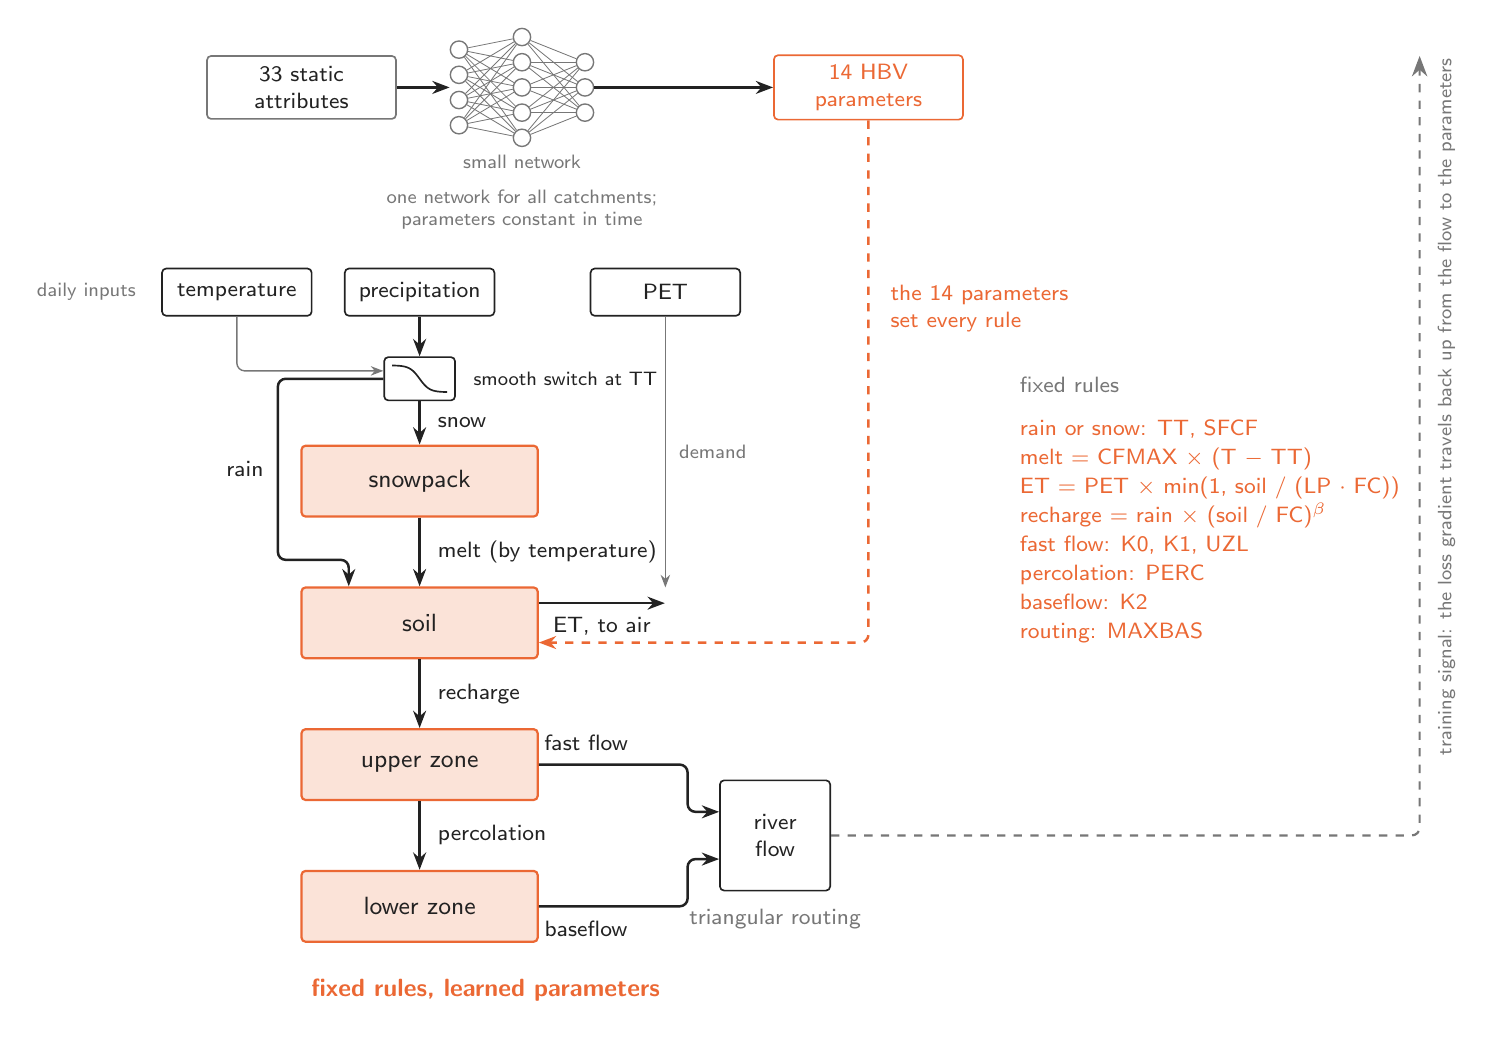
\begin{tikzpicture}[
  font=\sffamily\small, color=ink,
  store/.style={draw=model, fill=storefill, line width=0.8pt, minimum width=30mm, minimum height=9mm, rounded corners=1.5pt},
  flux/.style={-{Stealth[length=2.2mm]}, line width=0.9pt, color=ink, rounded corners=1mm},
  drives/.style={-{Stealth[length=1.6mm]}, line width=0.5pt, color=grey, rounded corners=1mm},
  lab/.style={font=\sffamily\footnotesize, color=ink, align=left},
  rule/.style={font=\sffamily\footnotesize, color=model, align=left},
  param/.style={-{Stealth[length=2.2mm]}, dashed, color=model, line width=0.9pt, rounded corners=1mm},
  grad/.style={-{Stealth[length=2.6mm]}, dashed, color=grey, line width=0.8pt, rounded corners=1mm},
  box/.style={draw=grey, line width=0.6pt, rounded corners=1.5pt, minimum height=8mm, align=center, font=\sffamily\footnotesize},
  input/.style={draw=ink, line width=0.6pt, rounded corners=1.5pt, minimum height=6mm, minimum width=19mm, align=center, font=\sffamily\footnotesize},
  neuron/.style={circle, draw=grey, fill=white, line width=0.5pt, minimum size=2.2mm, inner sep=0pt},
  switch/.style={draw=ink, line width=0.6pt, rounded corners=1.5pt, minimum width=9mm, minimum height=5.5mm, inner sep=1pt},
]
% ---- attributes -> a small network -> 14 parameters
\node[box, minimum width=24mm] (att) at (0, 0) {33 static\\attributes};
\foreach \i in {1,2,3,4} {\node[neuron] (i\i) at (20mm, {(2.5-\i)*3.2mm}) {};}
\foreach \i in {1,...,5}  {\node[neuron] (h\i) at (28mm, {(3-\i)*3.2mm}) {};}
\foreach \i in {1,2,3}    {\node[neuron] (o\i) at (36mm, {(2-\i)*3.2mm}) {};}
\foreach \i in {1,2,3,4} {\foreach \j in {1,...,5} {\draw[grey, line width=0.3pt] (i\i) -- (h\j);}}
\foreach \i in {1,...,5} {\foreach \j in {1,2,3} {\draw[grey, line width=0.3pt] (h\i) -- (o\j);}}
\node[lab, color=grey, font=\sffamily\scriptsize] at (28mm, -9.5mm) {small network};
\node[box, minimum width=24mm, draw=model, color=model] (par) at (72mm, 0) {14 HBV\\parameters};
\draw[flux] (att.east) -- (i2.west |- att.east);
\draw[flux] (o2.east) -- (par.west);
\node[lab, color=grey, font=\sffamily\scriptsize, align=center] at (28mm, -15.5mm) {one network for all catchments;\\parameters constant in time};

% ---- the daily inputs, one row
\node[input] (pin) at (15mm, -26mm) {precipitation};
\node[input, left=4mm of pin] (tin) {temperature};
\node[input, right=12mm of pin] (petin) {PET};
\node[lab, color=grey, font=\sffamily\scriptsize, left=2mm of tin] {daily inputs};

% ---- the store chain
\node[switch] (sw) at (15mm, -37mm) {};
\draw[ink, line width=0.6pt] plot[domain=-3.5:3.5, samples=30] ({15mm + \x*1mm}, {-37mm - 1.7mm + 3.4mm/(1+exp(\x*1.6))});
\node[lab, font=\sffamily\scriptsize, right=1mm of sw, align=left] {smooth switch at TT};
\node[store] (sp) at (15mm, -50mm) {snowpack};
\node[store] (sm) at (15mm, -68mm) {soil};
\node[store] (suz) at (15mm, -86mm) {upper zone};
\node[store] (slz) at (15mm, -104mm) {lower zone};
\draw[flux] (pin) -- (sw);
\draw[flux] (sw) -- (sp) node[midway, right=1mm, lab] {snow};
\draw[flux] (sw.west) -| (-3mm, -60mm) node[pos=0.75, left=0.5mm, lab] {rain} -| ($(sm.north)+(-9mm,0)$);
\draw[flux] (sp) -- (sm) node[midway, right=1mm, lab] {melt (by temperature)};
\draw[flux] ($(sm.east)+(0,2.5mm)$) -- ++(16mm,0) node[midway, below=0.5mm, lab] {ET, to air};
\draw[flux] (sm) -- (suz) node[midway, right=1mm, lab] {recharge};
\draw[flux] (suz) -- (slz) node[midway, right=1mm, lab] {percolation};
% what drives the switch and ET (thin grey)
\draw[drives] (tin.south) |- ($(sw.west)+(-3mm,1mm)$) -- ($(sw.west)+(0,1mm)$);
\draw[drives] (petin.south) -- ($(petin.south |- sm.east)+(0,4.5mm)$) node[pos=0.5, right=0.5mm, lab, color=grey, font=\sffamily\scriptsize] {demand};
% river
\node[box, draw=ink, minimum width=14mm, minimum height=14mm] (q) at ($(suz.east)!0.5!(slz.east)+(30mm,0)$) {river\\flow};
\draw[flux] (suz.east) -- ++(12mm,0) node[pos=0.5, above=0.5mm, lab] {fast flow} -| ($(q.west)+(-4mm,3mm)$) -- ($(q.west)+(0,3mm)$);
\draw[flux] (slz.east) -- ++(12mm,0) node[pos=0.5, below=0.5mm, lab] {baseflow} -| ($(q.west)+(-4mm,-3mm)$) -- ($(q.west)+(0,-3mm)$);
\node[lab, below=1mm of q, color=grey, align=center] {triangular routing};

% ---- the parameters feed the model: one arrow into the middle of the chain
\draw[param] (par.south) |- ($(sm.east)+(0,-2.5mm)$) node[pos=0.18, right=1.5mm, rule, align=left] {the 14 parameters\\set every rule};

% ---- the rules, in the model colour
\node[lab, color=grey, anchor=south west] at (90mm, -40mm) {fixed rules};
\node[rule, anchor=north west] at (90mm, -41mm) {%
  rain or snow: TT, SFCF\\[1pt]
  melt = CFMAX $\times$ (T $-$ TT)\\[1pt]
  ET = PET $\times$ min(1, soil / (LP $\cdot$ FC))\\[1pt]
  recharge = rain $\times$ (soil / FC)$^{\beta}$\\[1pt]
  fast flow: K0, K1, UZL\\[1pt]
  percolation: PERC\\[1pt]
  baseflow: K2\\[1pt]
  routing: MAXBAS};


\draw[grad] (q.east) -- (142mm, -95mm) -- (142mm, 4mm) node[pos=0.55, anchor=north, xshift=1mm, lab, color=grey, font=\sffamily\scriptsize, rotate=90] {training signal: the loss gradient travels back up from the flow to the parameters};
% ---- footer
\node[lab, color=model, font=\sffamily\small\bfseries, anchor=north west] at (0mm, -112mm) {fixed rules, learned parameters};
\end{tikzpicture}
\end{document}
